\documentclass[journal,12pt,twocolumn]{IEEEtran}

\usepackage{setspace}
\usepackage[cmex10]{amsmath}
\usepackage{amsthm}
\usepackage{mathrsfs}
\usepackage{enumitem}
\usepackage{mathtools}
\usepackage{graphicx}
\let\vec\mathbf

\newcommand{\mydet}[1]{\ensuremath{\begin{vmatrix}#1\end{vmatrix}}}
\newcommand{\myvec}[1]{\ensuremath{\begin{pmatrix}#1\end{pmatrix}}}
\providecommand{\brak}[1]{\ensuremath{\left(#1\right)}}

\title{Assignment 1}
\author{Varshini Jonnala (CS21BTECH11024)}


\begin{document}

        %The title
    \maketitle
        % The question
    \textbf{Question: }\\
      A(2,5), B(-1,2) and C(5,8) are the vertices of the triangle ABC, M is a point on AB such that AM:MB = 1:2. Find the co-ordinates of M. Hence find the equation of line passing through the points C and M.

    \textbf{Solution: }
     Given, $\vec{A}, \vec{B}, \vec{C}$ form a triangle $ABC$.
	\begin{align}
		\vec{A} = \myvec{2 \\ 5} ,
		\vec{B} = \myvec{-1 \\ 2},
		\vec{C} = \myvec{5 \\ 8}
	\end{align}
   Let 
    \begin{align}
        \overrightarrow{a} = \overrightarrow{OA}\\
        \overrightarrow{b} = \overrightarrow{OB}\\
        \overrightarrow{m} = \overrightarrow{OM}
    \end{align}
    and $\vec{M}$ divides $\overrightarrow{AB}$ internally in the ratio of k : 1
    Then, we get 
    \begin{align}
       \label{5} \overrightarrow{m}=\frac{k\overrightarrow{b}+1\overrightarrow{a}}{k+1}
    \end{align}

    Given, $\vec{M}$ is a point on side $AB$ such that $AM:MB = 1:2$. 
        Using \eqref{5}, we get
    \begin{align}
        \overrightarrow{m} = \frac{\overrightarrow{b}+2\overrightarrow{a}}{3}
    \end{align}
    On substituting, we get
    \begin{align}
        \vec{M} &= \frac{\myvec{-1 \\ 2} + 2\myvec{2 \\ 5}}{3}\\ \implies \vec{M} &= \myvec{1\\4}.
    \end{align}
    
    Let L be the line that passes through points $\vec{C}\myvec{5\\8}$,
    The direction vector of $CM$ is,
    
    \begin{align}
        &\vec{m} = \vec{C} - \vec{M}\\
	    \implies &\vec{m} = \myvec{5 \\ 8} - \myvec{1 \\ 4}\\
	    \implies &\vec{m} = \myvec{4 \\ 4}
    \end{align}
    
    Normal vector of the line is $\vec{n}$, such that
    \begin{align}
	    &\vec{m}^{\top}\vec{n} = 0\\
	    &\implies \myvec{4 & 4}\vec{n} = 0\\
	    &\implies \vec{n} = \myvec{1 \\ -1}\\
	    &\implies \vec{n}^{\top} = \myvec{1 & -1}
    \end{align}
    
    The normal equation of the line L is given by, 
    \begin{align}
	    &\vec{n}^{\top}\brak{\vec{x} - \vec{M}} = 0\\
	    \implies &\myvec{1 & -1}\brak{\vec{x} - \myvec{1 \\ 4}}= 0\\
	    \implies &\myvec{1 & -1}\vec{x} = -3
    \end{align}
    
    Thus, the equation of line $\vec{L}$ passing through  $\vec{C}\myvec{5\\8}$ and $\vec{M}\myvec{1\\4}$ is 
        
    \begin{align}
          \myvec{1 & - 1}\vec{x} + 3 &= 0
    \end{align}
        which can also be represented as 
    \begin{align}
         x-y+3=0
    \end{align}
      
    {\large But, However,} We get
    \begin{enumerate}
        \item The equation of the line joining $\vec{A}\myvec{2\\5}$, $\vec{B}\myvec{-1\\2}$ as $\myvec{1 & - 1}\vec{x} = -3$.
           
        \item The equation of the line joining $\vec{B}\myvec{-1\\2}$, $\vec{C}\myvec{5\\8}$ as $\myvec{1 & - 1}\vec{x}=-3$ too.
    \end{enumerate}
   
    Now, Let's find the area of triangle to verify if the points are collinear:
    Given, 
    \begin{align}
		\vec{A} = \myvec{2 \\ 5} ,
		\vec{B} = \myvec{-1 \\ 2},
		\vec{C} = \myvec{5 \\ 8}
	\end{align}
	are the vertices of triangle.
	\begin{align}
	\vec{A}-\vec{B} &= \myvec{3 \\3},\\
	\vec{A}-\vec{C} &= \myvec{-3 \\-3},
	\end{align}
	
	The desired area is  the magnitude of 
    \begin{align}
     \mydet{3 & -3\\3 & -3} 
    \end{align}
    Thus the desired area is 0 units.
	
    \large Hence, Given points $\vec{A}, \vec{B}, \vec{C}$ don't form a triangle.

    \large Also Verified by plotting the graph of $\vec{A}, \vec{B}, \vec{C}$ and $\vec{M}$ points :

    % The graph
  	\begin{figure}[!ht]
		\centering
		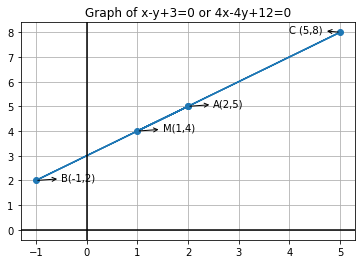
\includegraphics[width=\columnwidth]{prv1.png}
		\caption{\large Graph showing that the points  $\vec{A}, \vec{B}, \vec{C}$, $\vec{M}$ lie on the same line.}
	\end{figure}
	
\end{document}
